\section{Introducción}

%###########################
%######### Qubits ##########
\begin{frame}{Qubits y su dinámica}
    \begin{columns}
        \begin{column}{0.5\textwidth}
            \begin{center}
                Un qubit es un sistema cuántico de dos estados.
                \pause
                Todo qubit se puede escribir como
                \begin{equation}
                    \ket{\psi}=\alpha\ket{0}+\beta\ket{1}.\nonumber
                \end{equation}
                \pause
                Por convención usamos los eigenestados del operador $\pauli{3}$.
                \begin{align}
                    \ket{0} & & \text{y} & & \ket{1}. \nonumber
                \end{align} 
            \end{center}
        \end{column}
        \pause
        \begin{column}{0.5\textwidth}
            La evolución de un sistema cuántico descrito por $\ket{\psi}$ está dada por
            \begin{equation}
                \rmi\hbar\frac{d}{dt}\ket{\psi(t)}=H\ket{\psi(t)}.\nonumber
            \end{equation}
            \pause
            Cuya solución es una evolución unitaria $U(t,t_{0})=e^{-\rmi H(t-t_{0})/\hbar}$
            \begin{align}
                \ket{\psi(t)}=U(t,t_{0})\ket{\psi(t_{0})} \rlap{.}\nonumber
            \end{align}
        \end{column}
    \end{columns}
\end{frame}
\begin{frame}{Parametrización de un qubit}
    \begin{columns}
        \begin{column}{0.5\textwidth}
            Un qubit $\ket{\psi}\in\hilbert_{2}$ arbitrario
            \begin{equation}
                \ket{\psi}=\alpha\ket{0}+\beta\ket{1},\nonumber
            \end{equation}
            \pause
            se puede reescribir como:
            \begin{equation}
                \ket{\psi}=\cos(\frac{\theta}{2})\ket{0}+e^{\rmi\varphi}\sin(\frac{\theta}{2})\ket{1}.\nonumber
            \end{equation}
        \end{column}
        \begin{column}{0.5\textwidth}
            \centering
            \BlochSphere
        \end{column}
    \end{columns}
\end{frame}
%###########################


%###########################
%# Descripciones efectivas #
\begin{frame}{Dinámica que emerge de una descripción efectiva}
    \begin{center}
        ``Dinámica \textbf{efectiva} de un sistema de N qubits''
    \end{center}
    \pause
    \begin{columns}
        \begin{column}{0.5\textwidth}
            \begin{center}
                Dinámica \textbf{efectiva}\\
                \pause
                $\downarrow$\\
                Dinámica {\tiny(que emerge de una descripción)} \textbf{efectiva}
            \end{center}
            \pause
            Aquí, 
            \begin{center}
                \textit{efectiva}$\iff$\textit{gruesa}.
            \end{center}
        \end{column}
        \pause
        \begin{column}{0.5\textwidth}
            La descripción gruesa de un sistema es resultado de
            \begin{itemize}
                \item Aparato de medición imperfecto
                \item Descarte de grados de libertad del sistema
            \end{itemize}
        \end{column}
    \end{columns}
\end{frame}
\begin{frame}{Descripciones efectivas y modelos de grano grueso}
    \begin{center}
        Una descripción de grano grueso es aquella que no toma en cuenta todos los detalles de un sistema o fenómeno.
    \end{center}
    \pause
    \begin{columns}
        \begin{column}{0.5\textwidth}
            \begin{center}
                Variables termodinámicas\\
                $\downarrow$\\
                Descripción efectiva\\
                \pause
                \begin{equation}
                    T=\frac{1}{k_\text{B}}\frac{2}{3}\expval{E_{\text{cin}}}.\nonumber
                \end{equation}
            \end{center}
        \end{column}
        \begin{column}{0.5\textwidth}
            \begin{figure}
                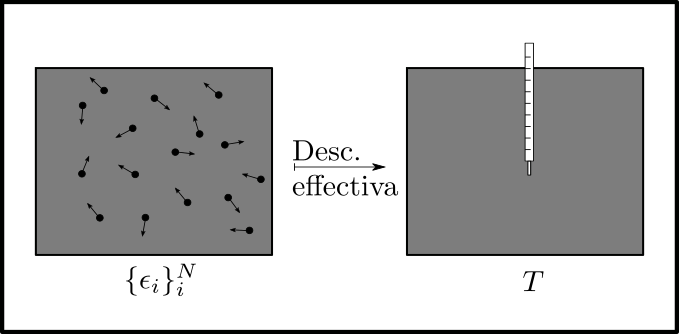
\includegraphics[width=1\textwidth]{figures/CGT.png}
            \end{figure}
        \end{column}
    \end{columns}
\end{frame}
%###########################


%###########################
% ## Operador de densidad ##
\subsection{El operador de densidad}

\begin{frame}{Mezclas estadísticas}
    \begin{columns}
        \begin{column}{0.5\textwidth}
            \begin{block}{Probabilidad cuántica}
            Los vectores de estado contienen probabilidad cuántica:
            \begin{equation}
                \ket{\psi}=\alpha\ket{0}+\beta\ket{1},\nonumber
            \end{equation}
            \pause
            de la que se recupera la regla de Born:
            \begin{equation}
                p(\ket{0})=\abs{\alpha}^{2}\qquad p(\ket{0})=\abs{\beta}^{2}\nonumber
            \end{equation}
        \end{block}
        \end{column}
        \pause
        \begin{column}{0.5\textwidth}
            \begin{block}{Probabilidad \textit{por ignorancia}}
            Un sistema del que se sabe se halla en el estado $\ket{\varphi_{j}}$ con probabilidad $p_{j}$.\\
            \vspace{0.2cm}
            \pause
            De este sistema se halla en un estado de \textit{mezcla estadística}.\\
            \vspace{0.2cm}
            \pause
            Es descrito por el operador de densidad
            \begin{equation}
                \rho=\sum_{j}p_{j}\dyad{\varphi_{j}}.\nonumber
            \end{equation}
        \end{block}
        \end{column}
    \end{columns}
\end{frame}
\begin{frame}{Parametrización}
    \begin{columns}
        \begin{column}{0.5\textwidth}
            Una base hermítica permite parametrizar a una matriz de densidad a través del producto punto de Hilbert-Schmidt
            \begin{equation}
                \rho=\frac{1}{2}\qty(\Id_{2}\Tr(\rho)+\sum_{k=1}^{3}\Tr(\rho\pauli{k})\pauli{k}).\nonumber
            \end{equation}
            \pause
            El vector de Bloch es
            \begin{equation}
                \vec{r}_{\rho}=\begin{pmatrix}
                    \Tr(\rho\pauli{x})\\
                    \Tr(\rho\pauli{y})\\
                    \Tr(\rho\pauli{z})
                \end{pmatrix}\nonumber
            \end{equation}
        \end{column}
        \pause
        \begin{column}{0.5\textwidth}
            \centering
            \BlochSphereDensity
        \end{column}
    \end{columns}
\end{frame}
%###########################


%###########################
%#### Sistemas abiertos ####
\begin{frame}{Sistemas multipartitos}
    \begin{columns}
        \begin{column}{0.5\textwidth}
            \begin{block}{Combinar y reducir}
            Si $\rho_{\text{bi}}$ describe dos qubits A y B,
            \begin{equation}
                \hilbert_{\text{bi}}=\hilbert_{2}\otimes\hilbert_{2}.\nonumber
            \end{equation}
           \pause
           ¿Qué sucede si es relevante \textbf{una} partícula?\pause
            \begin{equation}
                \rho^{A}=\Tr_{B}(\rho_{\text{bi}}),\nonumber
            \end{equation}
            \end{block}
        \end{column}
        \pause
        \begin{column}{0.5\textwidth}
            \begin{block}{Evolución}
            Sistema multipartito $\rightarrow$ von Neumann
            \begin{equation}
                \rmi\hbar\frac{d}{d t} \rho_{\text{bi}}(t)=[H,\rho_{\text{bi}}(t)].\nonumber
            \end{equation}\pause
            \vspace{0.3cm}
            Trazando:
            \begin{align}
                \rmi\hbar\frac{d}{d t} \rho^{A}(t)=\Tr_{B}([H,\rho_{\text{bi}}(t)])\rlap{.}\nonumber
            \end{align}
        \end{block}
        \end{column}
    \end{columns}
\end{frame}
\begin{frame}{Evolución abierta}
    Supóngase que el sistema de interés está acoplado a un \textit{entorno}: $\rho_{\text{Tot}}(0)=\rho_{S}(0)\otimes\rho_{E}$
    \begin{columns}
        \begin{column}{0.5\textwidth}
            \begin{block}{El canal cuántico}
            \begin{align}
                \rmi\hbar\frac{d}{d t} \rho_{S}(t)=\Tr_{E}([H,\rho_{\text{Tot}}(t)])\rlap{,}\nonumber
            \end{align}\pause
            Tiene solución:
            \begin{equation}
                \begin{gathered}
                \rho_{S}(t)=\mcE_{t}(\rho_{S}(0))\\
                \mcE_{t}(\rho_{S}(0))=\Tr_{E}\qty[U(t)\left(\rho_{S}(0)\otimes\rho_{E}\right)U^{\dag}(t)]
            \end{gathered}\nonumber
            \end{equation}
            \end{block}
        \end{column}
        \pause
        \begin{column}{0.5\textwidth}
            \begin{block}{Operadores de Kraus}
            \begin{itemize}
                \item $\mcE(\rho)=\sum_{k}A_{k}\rho A^{\dagger}_{k}$
                \item $\sum_{k}A_{k}^{\dagger}A_{k}=\Id$
            \end{itemize}
        \end{block}
        \end{column}
    \end{columns}
\end{frame}
%###########################



%###########################
%### Ejemplos de canales ###
\begin{frame}{Ejemplo de canal cuántico: desfasamiento}
    \begin{center}
        El \textit{canal de desfasamiento} tiene operadores de Kraus $\{\sqrt{p}\Id,\sqrt{(1-p)}\pauli{3}\}$.
    \end{center}
    \begin{figure}
        \centering
        \begin{subfigure}{0.45\textwidth}
            \centering
            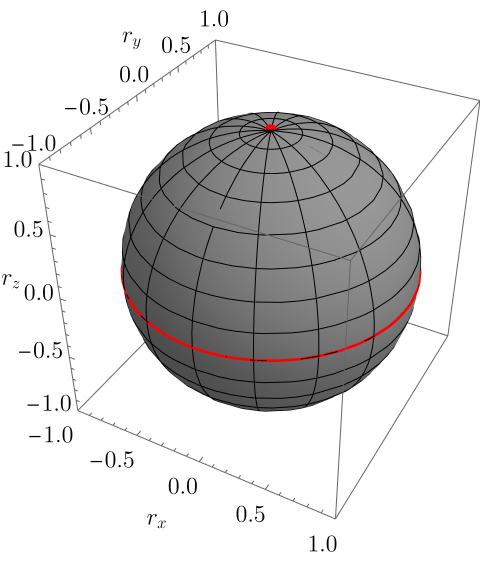
\includegraphics[width=0.5\textwidth]{figures/whole_sphere.png}
        \end{subfigure}
        \begin{subfigure}{0.45\textwidth}
            \centering
            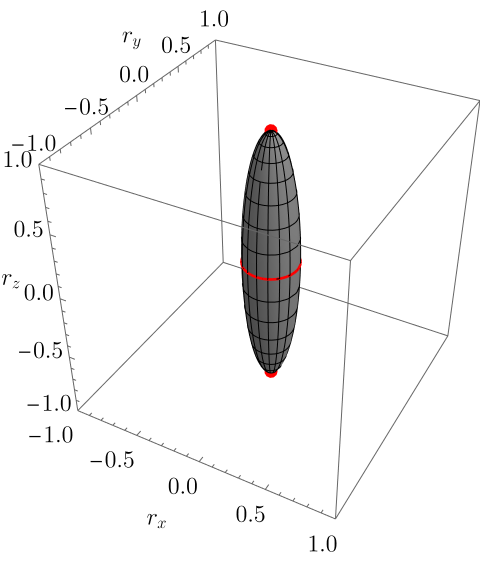
\includegraphics[width=0.5\textwidth]{figures/dephased.png}
        \end{subfigure}
    \end{figure}
\end{frame}
\begin{frame}{Ejemplo de canal cuántico: bitflip}
    \begin{center}
        El \textit{canal de bitflip} tiene operadores de Kraus $\{\sqrt{p}\Id,\sqrt{(1-p)}\pauli{1}\}$.
    \end{center}
    \begin{figure}
        \centering
        \begin{subfigure}{0.45\textwidth}
            \centering
            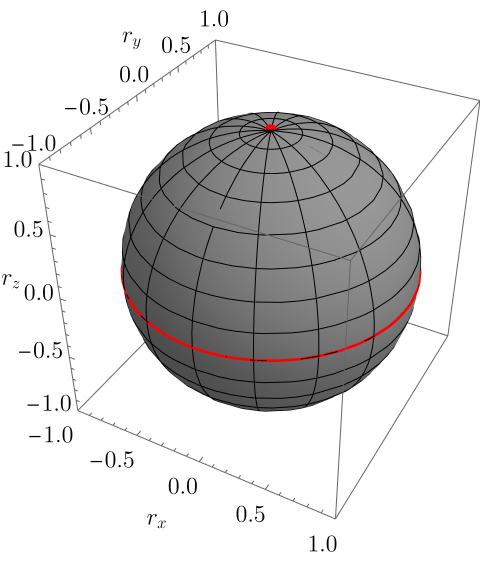
\includegraphics[width=0.5\textwidth]{figures/whole_sphere.png}
        \end{subfigure}
        \begin{subfigure}{0.45\textwidth}
            \centering
            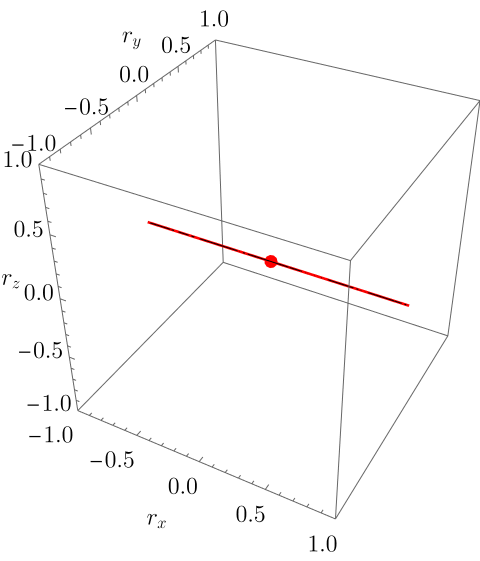
\includegraphics[width=0.5\textwidth]{figures/bitflip.png}
        \end{subfigure}
    \end{figure}
\end{frame}
\begin{frame}{Ejemplo de canal cuántico: despolarización}
    Finalmente, el \textit{canal de despolarización} se define mediante
    \begin{equation}
        \rho\mapsto p\frac{1}{2}\Id+(1-p)\rho\nonumber.
    \end{equation}
    \begin{figure}
        \centering
        \begin{subfigure}{0.45\textwidth}
            \centering
            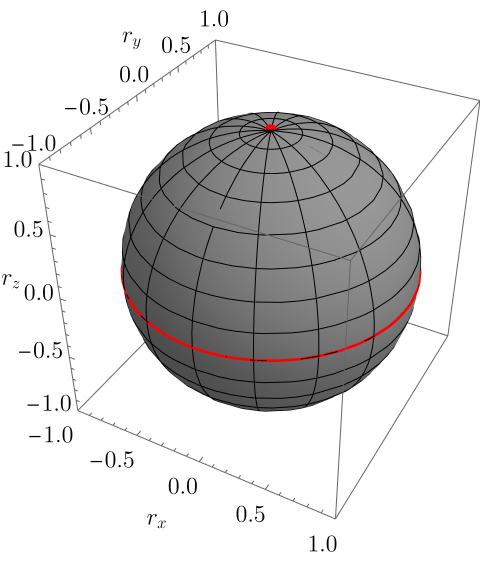
\includegraphics[width=0.5\textwidth]{figures/whole_sphere.png}
        \end{subfigure}
        \begin{subfigure}{0.45\textwidth}
            \centering
            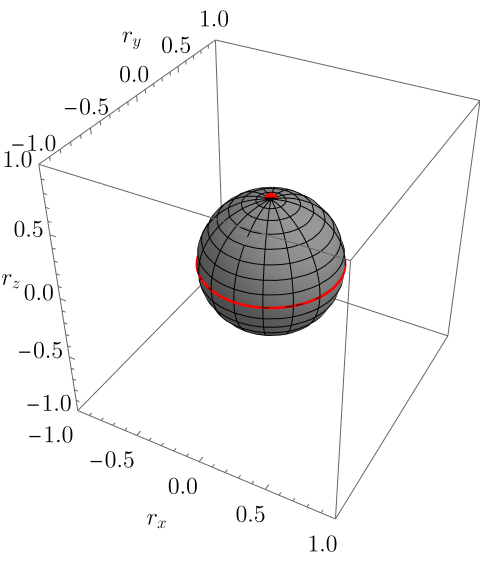
\includegraphics[width=0.5\textwidth]{figures/depol.png}
        \end{subfigure}
    \end{figure}
\end{frame}
%###########################

\begin{frame}{El problema: motivación}
    \begin{center}
        Se estudia la dinámica que emerge de una descripción efectiva
    \end{center}
    \begin{columns}
        \begin{column}{0.5\textwidth}
            \begin{displaymath}
                \xymatrix{
                  {\rho_{\ef}(0)} \ar[rr]^{\text{\textcolor{red}{?}}}
                  && {\rho_{\ef}(t)}\\
                  {\varrho_{\text{\textcolor{red}{?}}}(0)} \ar[rr]^{\mcE_{t}} \ar[u]^{\mcC}
                  && {\varrho_{\text{\textcolor{red}{?}}}(t)} \ar[u]^{\mcC}
                }
              \end{displaymath}
        \end{column}
        \pause
        \begin{column}{0.5\textwidth}
            \begin{displaymath}
                \xymatrix{
                  {\rho_{\ef}(0)} \ar[rr]^{{\mcC\circ\mcE_{t}\circ\color{red}\mcA}} \ar[d]^{{\color{red}\mcA}}
                  && {\rho_{\ef}(t)}\\
                  {\varrho_{{\color{red}\mcA}}(0)} \ar[rr]^{\mcE_{t}}
                  && {\varrho_{{\color{red}\mcA}}(t)} \ar[u]^{\mcC}
                }
              \end{displaymath}
              \pause
        \end{column}
    \end{columns}
    \begin{center}
        ¿Cómo construir ${\color{red}\mcA}$?
    \end{center}
\end{frame}

%###########################
%#### Entropía y MaxEnt ####
\subsection{Entropía e información}

\begin{frame}{Entropía en teoría de información clásica}
    \begin{columns}
        \begin{column}{0.5\textwidth}
            \begin{block}{Información clásica}
            \begin{center}
                A cada evento se le puede asociar una cantidad de información\pause
            \end{center}
            \begin{itemize}
                \item ``No cayó 6''$\rightarrow$poca información\pause
                \item ``Cayó 6''$\rightarrow$más información\pause
            \end{itemize}
            Entonces es decreciente con la probabilidad, monótona y Un evento $p=1$ no transmite información.
        \end{block}
        \end{column}
        \pause
        \begin{column}{0.5\textwidth}
            \begin{block}{Entropía de Shannon}
            Si , entonces debe poder calcularse la cantidad de información promedio:\\
            \pause
            Claude Shannon demostró 
            \begin{equation}
                S_{\text{S}}=-k\sum_{j}p(x_{j})\log{p(x_{j})}.\nonumber
            \end{equation}
        \end{block}
        \end{column}
    \end{columns}
\end{frame}

\subsection{El Principio de Máxima Entropía}

\begin{frame}{Intuición del Principio de Máxima Entropía}
    \begin{columns}
        \begin{column}{0.5\textwidth}
            \begin{block}{Usando dados: {\usefont{U}{dice3d}{m}{n}6a 2b 3d}}
                \begin{center}   
                Supóngase que $\expval{\text{\Pisymbol{dice3d}{102}}}=3.5$\\
                ¿$p(x)$?\\ \pause
                Dado balanceado:
                \begin{tabular}{ c c c }
                    $p(\epsdice{1})=\frac{1}{6}$ & $p(\epsdice{2})=\frac{1}{6}$ & $p(\epsdice{3})=\frac{1}{6}$ \\
                    $p(\epsdice{4})=\frac{1}{6}$ & $p(\epsdice{5})=\frac{1}{6}$ & $p(\epsdice{6})=\frac{1}{6}$
                \end{tabular}\pause \\
                \vspace{0.3cm}
                Dado pesado:
                \begin{tabular}{ c c c }
                    $p(\epsdice{5})=\frac{1}{2}$ & $p(\epsdice{2})=\frac{1}{2}$ & $p(\epsdice{1})=0$ \\
                    $p(\epsdice{3})=0$ & $p(\epsdice{4})=0$ & $p(\epsdice{6})=0$
                \end{tabular}
                \end{center}
            \end{block}
        \end{column}
        \begin{column}{0.5\textwidth}
            El principio de máxima entropía fue introducido por E. T. Jaynes en 1957.
            Jaynes afirma que la distribución de probabilidad que maximice la entropía es la estimación menos sesgada que se puede hacer.
        \end{column}
    \end{columns}
\end{frame}
\begin{frame}{El Principio de Máxima Entropía clásico}
    Sean $x_{j}$ los valores de $X$, $f_{k}$, funciones de valor esperado conocido. Maximizamos la entropía:
    \begin{equation}
        \mcL=-S_{\text{S}}(p)+\sum_{l}\lambda_{l}\qty(\sum_{j}p(x_{j})f_{l}(x_{j})-\expval{f_{l}(x)})+\mu\qty(\sum_{j}p(x_{j})-1).\nonumber
    \end{equation}
    Se deriva, se iguala a cero, se halla un sistema de ecuaciones. La distribución de probabilidad que maximiza la entropía: 
    \begin{equation}
        p(x_{j})=\frac{1}{Z}\exp[-\frac{1}{k}\sum_{l}\lambda_{l}f_{l}(x_{j})].\nonumber
    \end{equation}
\end{frame}
\begin{frame}{El Principio de Máxima Entropía cuántico}
    Usamos la entropía de von Neuman $S=-Tr(\rho\ln(\rho))$, que para $\rho$ $H$ tales que $[\rho,H]=0$ es
    \begin{equation}
        S_{\text{N}}=-\sum_{k}\eta_{k}\log{\eta_{k}}.\nonumber
    \end{equation}
    Siguiendo el mismo procedimiento, las soluciones:
    \begin{equation}
        \eta_{k}=-e^{(\lambda_{0}+1+\lambda_{1}E_{k})}=\frac{1}{Z}e^{-\lambda E_{k}}.\nonumber
    \end{equation}
    Utilizando notación de Dirac, $\rho=\sum_{k}\eta_{k}\dyad{e_{k}}$:
    \begin{equation}
        \rho=\frac{1}{Z}e^{-\lambda H}.\nonumber
    \end{equation}
    En general:
    \begin{equation}\label{eq:GeneralMaxEnt}
        \rho=\frac{1}{Z}e^{-\sum_{k}\lambda_{k} A_{k}}.\nonumber
    \end{equation}
\end{frame}
%###########################


%###########################
%###########################
\begin{frame}{El problema}
    \begin{center}
        ``Dinámica efectiva de un sistema de N qubits\\
        Utilizando el Principio de Máxima Entropía''
        \begin{displaymath}
            \xymatrix{
              {\rho_{\ef}(0)} \ar[rr]^{\Gamma_{t}} \ar[d]^{\mcA_{\mcC}^{\max}}
              && {\rho_{\ef}(t)}\\
              {\varrho_{\max}(0)} \ar[rr]^{\mcE_{t}}
              && {\varrho_{\max}(t)} \ar[u]^{\mcC}
            }
          \end{displaymath}
    \end{center}
\end{frame}
%###########################